%-----------------------------------------------------------
% Phantom-Head Modeling
%-----------------------------------------------------------
\begin{figure}[h]
    \centering
    \begin{subfigure}[b]{0.4\textwidth}
        \centering
        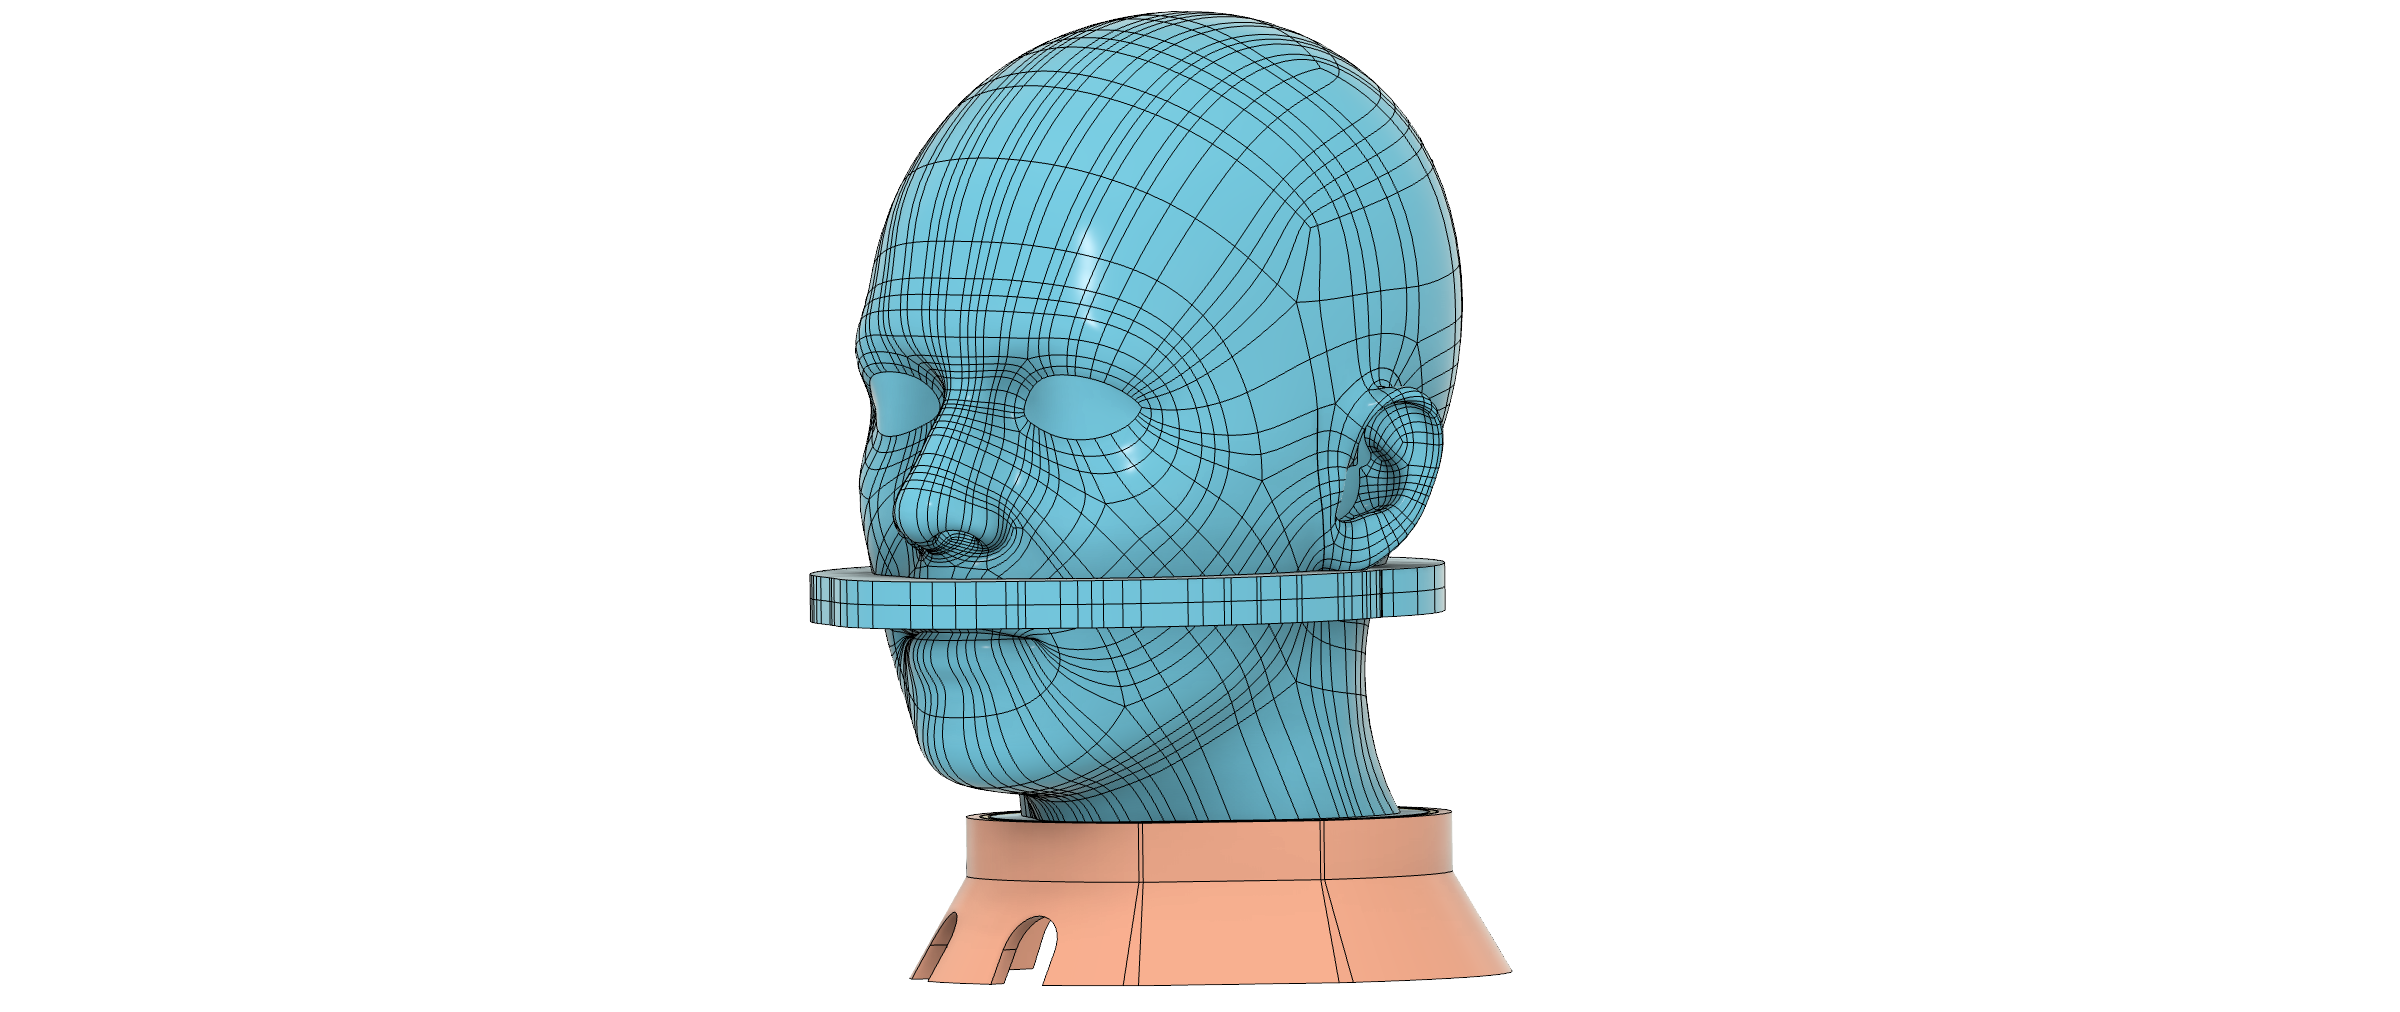
\includegraphics[width=\textwidth]{../../02_Images/3dmodel_overview.png}
        \caption[Phantom assembly exterior]{External overview of the phantom head assembly.}
        \label{fig:head_overview_complete}
    \end{subfigure}
    \hfill
    \begin{subfigure}[b]{0.4\textwidth}
        \centering
        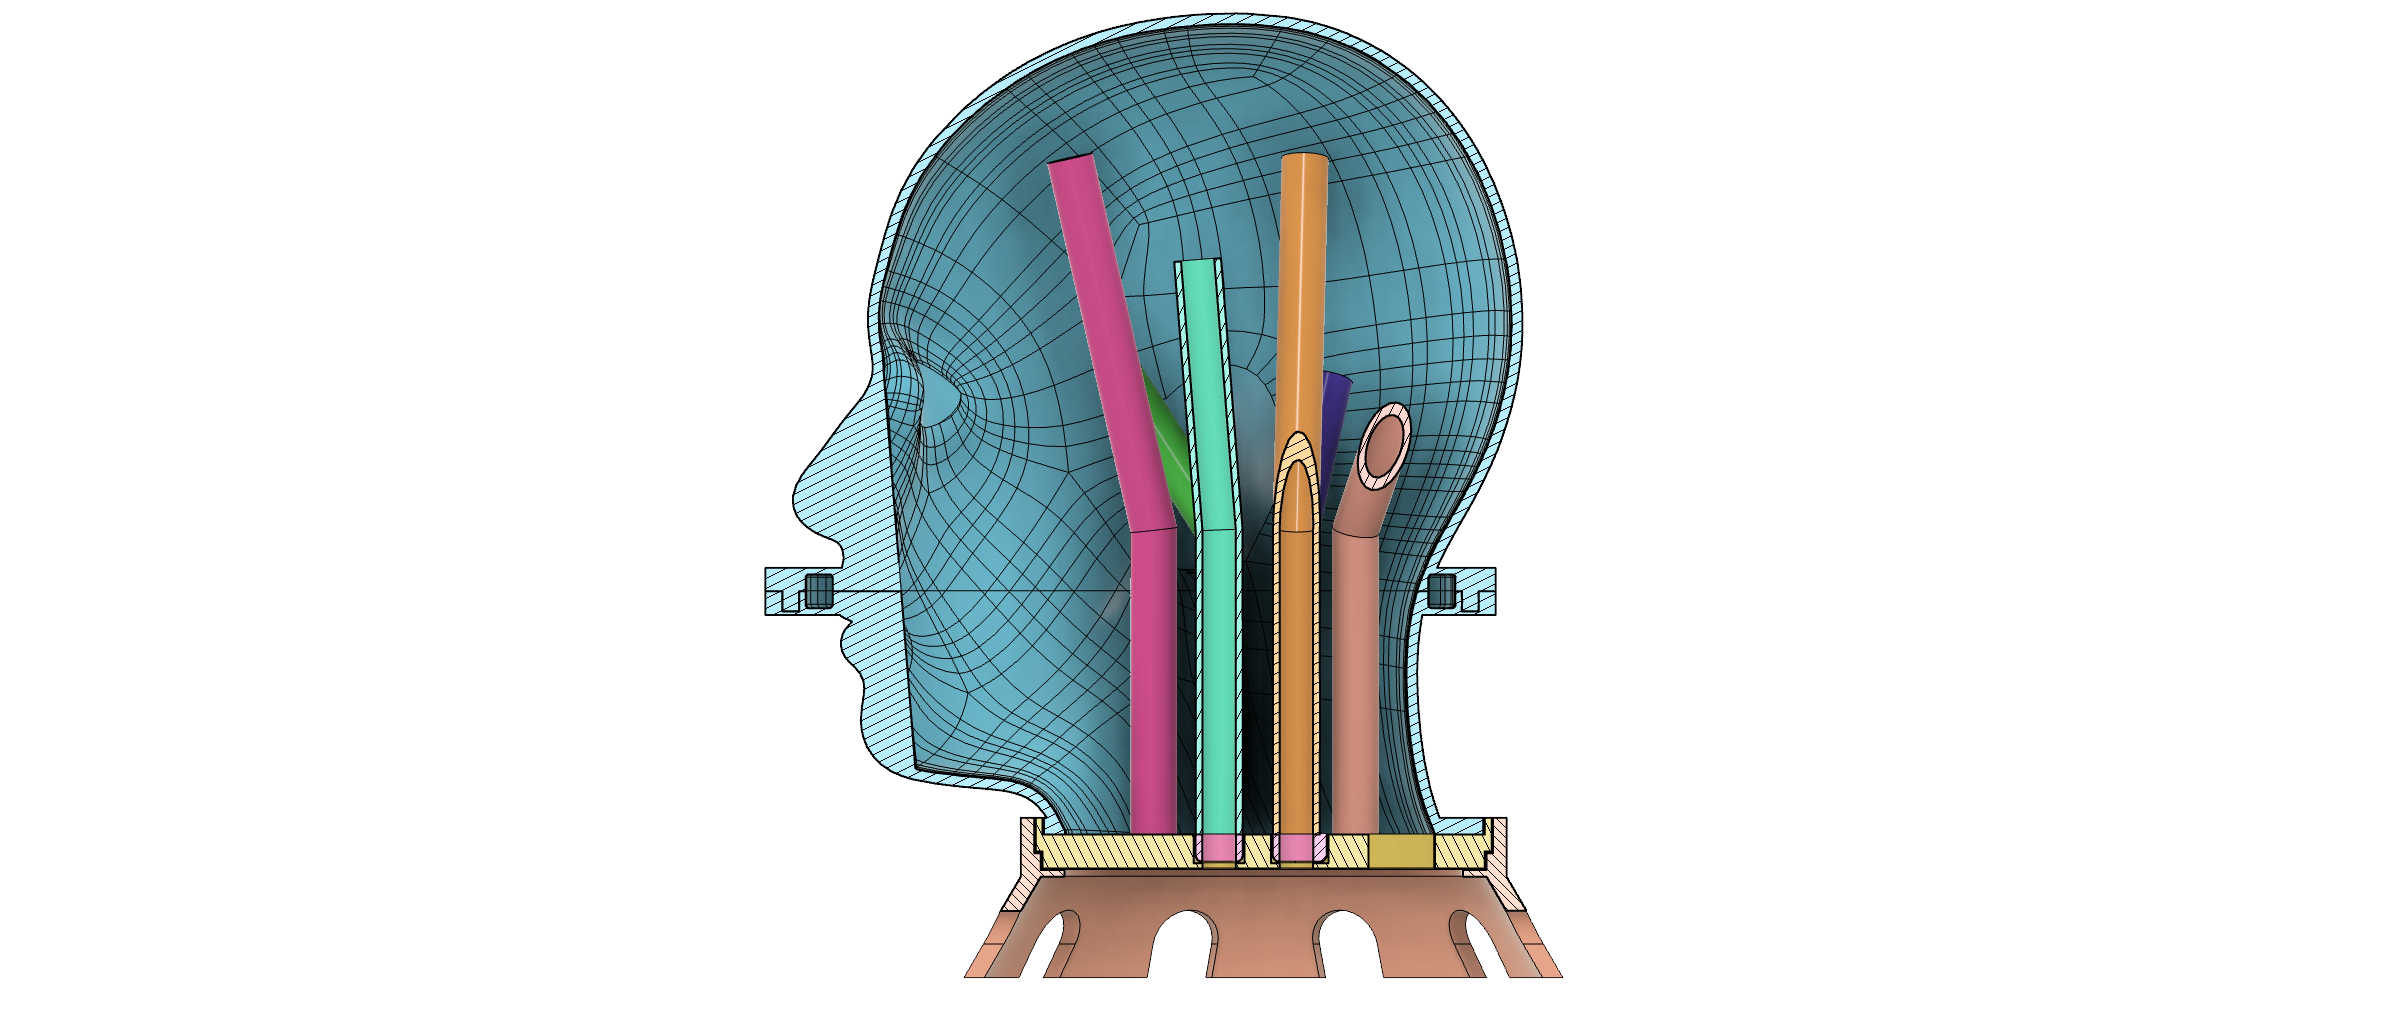
\includegraphics[width=\textwidth]{../../02_Images/3dmodel_section.png}
        \caption[Phantom assembly section]{Section analysis showing internal component disposition.}
        \label{fig:head_overview_section}
    \end{subfigure}
    \caption[Phantom head 3D model]{3D model of the phantom head, highlighting major components and internal structure.}
    \label{fig:head_overview}
\end{figure}

The phantom head model was developed to provide a realistic and modular platform 
for simulating electrical propagation through cranial tissues. 

A realistic mannequin head and torso geometry was sourced from the GrabCAD 
Community Library~\cite{grabcad}. The specific CAD model~\cite{mannequin-model} 
was then imported into \textit{Autodesk Fusion~360} for geometric processing and adaptation.

The phantom assembly was conceived as a modular system. The main components are:

\begin{itemize}
    \item a two-part outer \textbf{head shell} representing the skull boundary and defining the internal cavity to be filled with conductive material,
    \item a set of nine internal \textbf{wire guides} routed toward predefined internal coordinates,
    \item a \textbf{lid} featuring keyed openings for the placement and alignment of the wire guides, and
    \item a \textbf{support base} that seats the lid, provides mechanical stability for the assembly, and includes pass-through openings for routing external cables or connections beneath the phantom.
\end{itemize}


A central principle in the phantom’s design is modularity — the capacity to replace, extend, or reconfigure individual components without rebuilding the entire system. This flexibility is essential for experimental workflows, where electrode layouts, internal coordinates, or stimulation approaches may change between studies. The phantom therefore supports a wide range of experimental configurations and can be easily adapted by other researchers who wish to explore alternative wire-guide layouts, modify the number of guides, or introduce custom access features.

Two aspects of the physical design enable this modularity:

\begin{itemize}
    \item \textbf{Connector base geometry:}  
    The raw parametric model of the connector base for wire guides is provided as a standalone component. New wire guides can be generated by extending this base with a custom tube geometry leading to any desired internal coordinate. This makes it possible to produce alternative guide networks without altering the head shell or the remaining assembly.

    \item \textbf{Interchangeable lid:}  
    An empty version of the inferior lid is included, containing only the mating interface with the shell. Researchers may modify this lid to implement arbitrary numbers of openings or layouts while preserving compatibility with the rest of the phantom.
\end{itemize}
